% -*- root: ../main.tex -*-
\chapter{Design di Dettaglio}

\section{Design Gestione Cibo e Acqua}
    Per l'automatizzazione e la gestione di cibo e acqua si è partiti dalle user-stories e dal modello del dominio costruito per sviluppare l'applicativo desiderato. Osservando i requisiti è stato progettato il modello fisico e l'interazione dell'animale con esso. 
    Si riporta di seguito il \textbf{design del prototipo fisico}, con i sensori e attuatori in giallo e la spiegazione del suo funzionamento [Fig. \ref{fig:ciboacqua}].
    Il design permette la modularità tra cibo e acqua, scegliendo all'occorrenza solo uno dei due o entrambi.
    \begin{figure}[H]
        \caption{Design Prototipo Cibo e Acqua (sensori e attuatori in giallo)}
        \label{fig:ciboacqua}
        \centering
        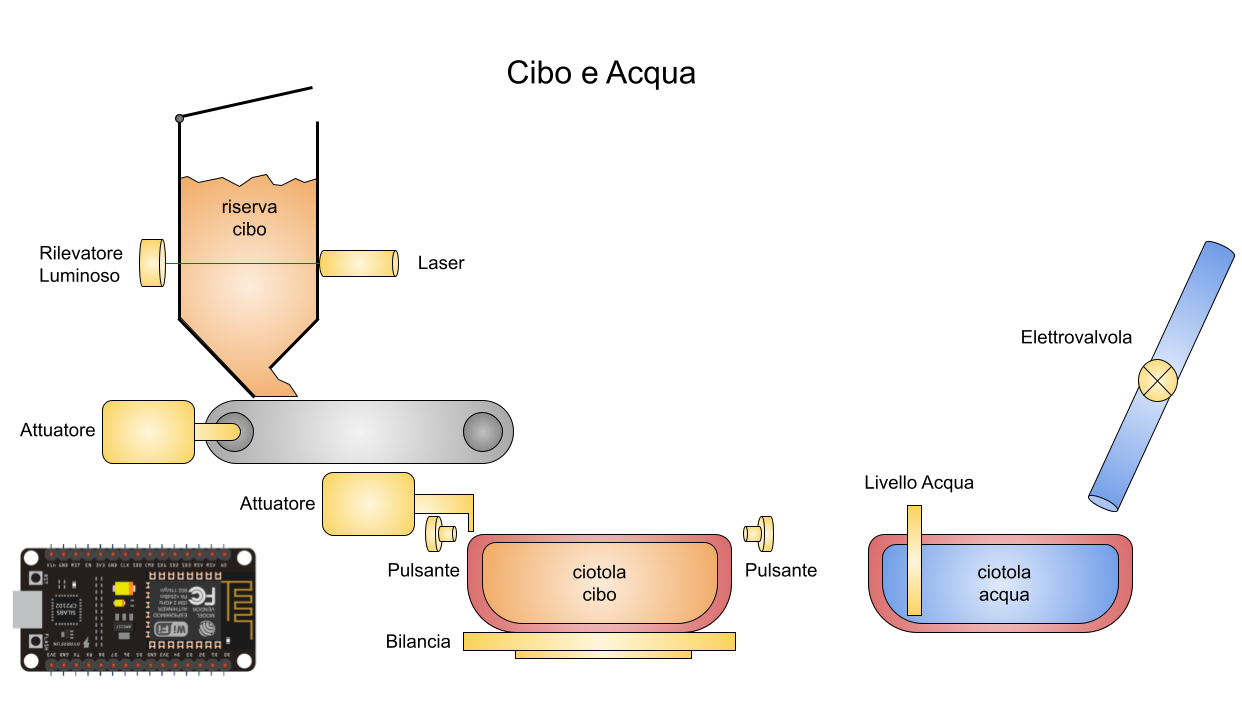
\includegraphics[width=1\textwidth]{Images/CiboAcqua.png}
    \end{figure}
    
    \subsection{Acqua}
    Per far fronte alla misurazione dei consumi, è stato innanzitutto necessario scegliere un sensore per ricavarne il \textbf{livello del liquido} [Fig. \ref{fig:ciboacqua}]. Il sensore deve ritornare un valore proporzionale alla percentuale di liquido rimanente. I consumi dell'animale a questo punto verranno inviati in cloud.
    
    Per quanto riguarda l'esigenza di riempimento dell'acqua, inizialmente la scelta era ricaduta su due sensori che rivelassero quando il liquido è al minimo o al massimo. In seguito questo design è stato semplificato usando direttamente il sensore introdotto per l'invio dei dati relativi al livello del liquido. 
    Successivamente è necessario che il sensore si interfacci con un'\textbf{elettrovalvola} [Fig. \ref{fig:ciboacqua}] per poter riempire la ciotola aprendo o chiudendo il flusso d'acqua all'occorrenza. 
    
    Il sistema deve essere modulare per design: qualora non si disponga del sistema idrico per poter rifornire la ciotola, devono comunque essere mandati i consumi con l'aggiunta di una notifica se se l'acqua sta per terminare.
    
    \subsubsection{Macchina a stati} Il comportamento è stato modellato come una macchina a stati [Fig. \ref{fig:statediagramWater}]. Ciò ha permesso di chiarire meglio le azioni del sistema a fronte di un avvenimento, il suo stato corrente e il suo comportamento generale.
    
    Inizialmente il comportamento prevede il controllo del \textbf{consumo di acqua}, ciclicamente e a intervalli regolari viene fatta una misurazione [Fig. \ref{fig:statediagramWater} "check water consumption"]. 
    
    E' stata stabilita una soglia minima di diminuzione del liquido per non incorrere in falsi positivi, dove le naturali oscillazioni del sensore potrebbero inviare consumi inesistenti. Talora questa soglia venisse superata, la \textbf{percentuale} di liquido consumata viene \textbf{inviata} in cloud, memorizzando l'ultima percentuale inviata [Fig. \ref{fig:statediagramWater} "send water consumption"]. Il sistema continua quindi a monitorare di nuovo il livello per ulteriori consumi. 
    
    Inevitabilmente il liquido nella ciotola andrà a finire, questo evento innescherà una transizione, dipendente dalla presenza o meno dell'elettrovalvola. 
    Se il sistema non prevede un rifornimento idrico il sistema passerà allo stato di \textbf{notifica di acqua esaurita} [Fig. \ref{fig:statediagramWater} "finished water notify"]. In questo stato una notifica verrà mandata all'addetto ai rifornimenti. Quando la ciotola verrà ricaricata il sistema passerà in automatico nuovamente allo stato per il controllo dei consumi.
    Qualora il sistema fosse dotato di elettrovalvola, la transizione innescata la aprirebbe, passando allo stato di \textbf{riempimento} [Fig. \ref{fig:statediagramWater} "fill water bowl"]. 
    
    In questo stato il livello viene controllato continuamente, per non incorrere in allagamenti indesiderati. 
    Un meccanismo di sicurezza temporizzato infatti controlla se un determinato periodo di tempo è passato senza che il sistema sia riuscito a riempire la ciotola con la valvola aperta. In caso affermativo il sistema va in blocco, chiudendo la valvola e passando allo stato di \textbf{notifica di errore} [Fig. \ref{fig:statediagramWater} "water system error notify"]. 
    Se il livello dell'acqua raggiunge il parametro desiderato invece lo stato torna a essere quello iniziale di osservazione.
    
    \begin{figure}[H]
        \caption{Macchina a Stati Acqua}
        \label{fig:statediagramWater}
        \centering
        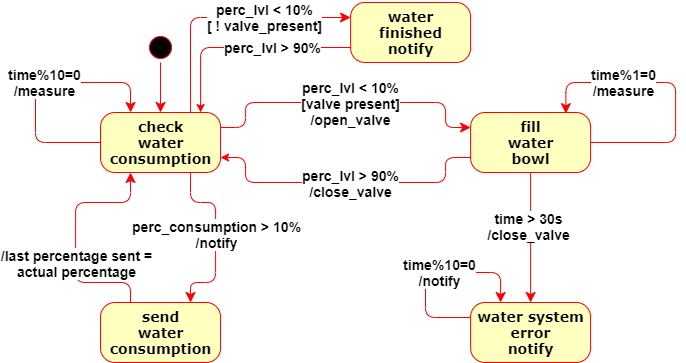
\includegraphics[width=1\textwidth]{DrawIo/stateDiagramWater.png}
    \end{figure}
    
    
    
    \subsection{Cibo}
    Per far fronte all'esigenza di monitorare i consumi di cibo dell'animale è stata introdotto un \textbf{sensore di peso} [Fig. \ref{fig:ciboacqua}]. Il sensore deve ritornare un valore proporzionale alla quantità di cibo presente nella ciotola. I consumi dell'animale verranno inviati in cloud. 
    
    Riguardo all'esigenza di rifornire il cibo, la bilancia si deve interfacciare con un attuatore che si occuperà della \textbf{distribuzione del materiale} [Fig. \ref{fig:ciboacqua} attuatore di sinistra]. Il design meccanico scelto è stato quello di un nastro trasportatore per la semplicità di realizzazione e l'efficacia. Altri design presi in esame comprendevano una botola che si aprisse e chiudesse, ma presentava problemi di forza per trattenere il cibo in caduta, e la vite di Archimede, ma presentava problemi nell'incastrarsi nel meccanismo dell'eventuale cibo in pezzi solidi. Il design con il nastro sfrutta la gravità per far cadere i pezzi su di esso e, all'attivazione, trascinarli con se permettendo ad altri di cadere. 
    La bilancia rileverà l'incremento e fermerà il sistema alla quantità desiderata.
    
    Per evitare che l'animale mangi il cibo durante la distribuzione, falsandone le misure, è stato introdotto un altro \textbf{attuatore bidirezionale} [Fig. \ref{fig:ciboacqua}] per estendere o ritrarre uno sportellino che ne previene l'accesso.
    Per determinare quando lo sportellino arriva al massimo o al minimo della sua estensione sono stati introdotti \textbf{due pulsanti} [Fig. \ref{fig:ciboacqua}] che segnalano quando fermare il movimento. 
    
    Infine per segnalare quando il cibo di scorta sta anch'esso per finire sono stati introdotti un \textbf{laser e un sensore luminoso} [Fig. \ref{fig:ciboacqua}] nella riserva di cibo. Se il cibo è presente il fascio laser verrà interrotto e il sensore non rileverà alcuna luce. Quando il cibo durante l'erogazione scende sotto una soglia critica, il fascio raggiunge il dispositivo di sensing e una notifica verrà inviata all'addetto. 
    
    Anche qui il sistema deve essere modulare per design: qualora non ci si voglia avvalere del sistema per rifornire la ciotola, i consumi devono comunque essere mandati in cloud con l'aggiunta di una notifica se il cibo nella ciotola sta per terminare.
    
    \subsubsection{Macchina a stati} Anche in questo caso il comportamento, data la sua complessità, è stato modellato come una \textbf{macchina a stati} [Fig. \ref{fig:statediagramFood}]. Il comportamento è simile alla macchina a stati mostrata in precedenza, essendo l'attuatore per il rifornimento del cibo paragonabile all'elettrovalvola e la bilancia paragonabile al sensore di livello dell'acqua. 
    
    Inizialmente il comportamento prevede il \textbf{controllo dei consumi} in maniera ciclica tramite la bilancia [Fig. \ref{fig:statediagramFood} "check food consumption"].
    Anche in questo caso talora la soglia minima venisse superata, la \textbf{quantità consumata viene inviata} in cloud [Fig. \ref{fig:statediagramFood} "send food consumption"]. Il sistema continua quindi a monitorare di nuovo il peso per ulteriori consumi.
    
    Se è stato scelto di non usufruire della parte di rifornimento cibo, il sistema quando questo si verrà ad esaurire, passerà allo \textbf{stato di notifica} [Fig. \ref{fig:statediagramFood} "food finished notify"]. Similmente al comportamento del sistema per l'acqua , quando la ciotola verrà ricaricata il sistema passerà in automatico nuovamente allo stato per il controllo dei consumi.
    In caso fosse presente il sistema di ricarica cibo completo, l'attuatore per chiudere l'accesso al cibo si attiverà, passando allo \textbf{stato di chiusura} [Fig. \ref{fig:statediagramFood} "blocking food access"]. Una volta completata la chiusura il nastro per l'erogazione del cibo verrà attivato e il sistema passerà allo \textbf{stato di erogazione} [Fig. \ref{fig:statediagramFood} "fill food bowl"]. Se non fosse presente lo sportellino per l'accesso al cibo, dallo stato iniziale si passerà direttamente a quest'ultimo attivando il nastro, senza il passaggio intermedio. 
    
    In questo stato il livello viene controllato continuamente, per un dosaggio corretto. Assieme al peso del cibo erogato, viene controllata anche la presenza del fascio laser. Qualora venisse rilevato significa che il cibo di scorta sta per finire e una notifica viene inviata all'addetto.
    Anche in questo caso è presente un meccanismo di sicurezza temporizzato che, dopo un periodo di tempo massimo, blocca l'erogazione e \textbf{passa allo stato di notifica errore} di sistema [Fig. \ref{fig:statediagramFood} "food system error notify"]
    
    In caso il cibo invece raggiunga la quantità desiderata, il sistema tornerà allo stato iniziale, garantendo eventualmente l'accesso al cibo tramite lo \textbf{stato di apertura} [Fig. \ref{fig:statediagramFood} "allowing food access"]    
    
    \begin{figure}[H]
        \caption{Macchina a Stati Cibo}
        \label{fig:statediagramFood}
        \centering
        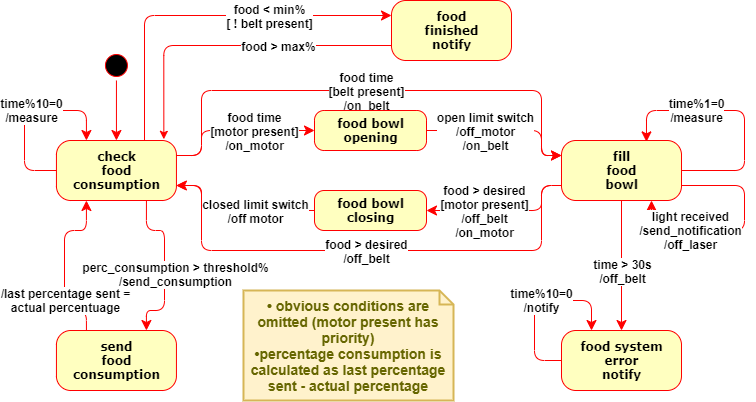
\includegraphics[width=1\textwidth]{DrawIo/stateDiagramFood.png}
    \end{figure}
    
    
\section{Design Monitoraggio Parametri Vitali}

\section{Design Videosorveglianza}

\section{Design del Database}
Per immagazzinare i dati necessari all'applicazione si è deciso di utilizzare \textbf{Dynamo DB}.
Il database principale doveva immagazzinare:
\begin{itemize}
    \item I \textbf{profili} dei \textbf{cani} presenti all'interno del canile;
    \item Gli \textbf{orari} e le \textbf{quantità} di cibo da somministrare a seconda del cane;
    \item I \textbf{valori} rilevati dai dispositivi di \textbf{sensing}, che comprendono:
    \begin{itemize}
        \item Temperatura corporea;
        \item Frequenza cardiaca;
        \item Consumo di acqua; 
        \item Consumo di cibo;
        \item Temperatura ambientale del canile;
        \item Umidità rilevata all'interno del canile;
    \end{itemize}
    \item I profili degli \textbf{utenti}.
\end{itemize}

La progettazione del database è stata portata a termine seguendo diversi passaggi:
    \begin{enumerate}
        \item Definizione di uno schema \textbf{ER} da utilizzare come base di partenza;
        \item Individuazione degli \textbf{accessi} mediante la definizione delle \textbf{query} principali;
        \item Definizione dei \textbf{pattern} di Primary Key e Sort Key;
        \item Aggiunta di un \textbf{ global index};
    \end{enumerate}
    
    \subsection{Definizione di un ER}
    Nonostante non si tratti di un database relazionale, abbozzare uno schema Entity Relationship può essere utile per avere una buona visione di partenza di come devono essere gestiti i dati.
    \subsubsection{Informazioni sui cani}
    Il primo schema ad essere stato elaborato è stato quello che racchiude tutto ciò che ha a che fare con i dati di un cane, ovvero il profilo del cane, i dettagli della sua relativa distribuzione del cibo e le rilevazioni di cibo, acqua, temperatura e battiti che lo riguardano.
     \begin{figure}[H]
        \caption{ER dati del cane}
        \label{fig:dogER}
        \centering
        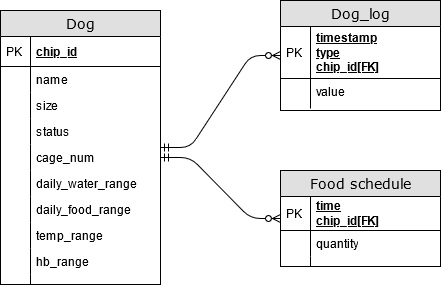
\includegraphics[width=0.6\textwidth]{DrawIo/EntityRelationship.png}
    \end{figure}
    \begin{itemize}
            \item \textbf{Cane}: il profilo del cane è modellato mediante la tabella \texttt{Dog} che, oltre alle consuete informazioni presenta anche le soglie, impostate dal veterinario, al di fuori delle quali si rileva un'anomalia.   
            
            \item \textbf{Programma dei pasti}: l'entità \texttt{Food\_Schedule} immagazzina gli orari e le quantità dei pasti. Il criterio secondo cui, nel caso standard, vengono decisi questi dati è la taglia, tuttavia si è deciso di collegare l'entità direttamente al cane poiché ciò permette di effettuare una programmazione più a grana fine. In questo modo, infatti, si può consentire ad un veterinario di effettuare modifiche sul regime alimentare di un unico cane, senza influenzare gli altri cani della stessa taglia.
            
            \item \textbf{Rilevazioni}: nello schema in figura è già stata collassata la gerarchia delle rilevazioni sopra elencate, concentrandole nell'entità \texttt{Dog\_log} che ne distingue la natura mediante il campo \texttt{type}.
       \end{itemize}
     \subsubsection{Informazioni sugli utenti}
     In fase di progettazione si voleva che il database gestisse anche gli utenti che agiscono sul sito, in maniera tale che ne fossero definiti i ruoli in base ai quali avrebbero avuto diversi permessi e una diversa visualizzazione dei dati sul sito web.
     Questo ER si distacca da quello relativo ai cani e si presenta in questo modo:
         \begin{figure}[H]
        \caption{ER utenti}
        \label{fig:userER}
        \centering
        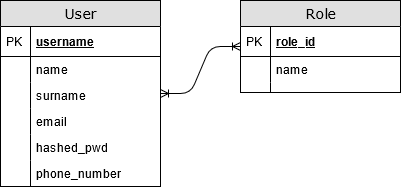
\includegraphics[width=0.6\textwidth]{DrawIo/UserER.png}
    \end{figure}
    
    \subsubsection{Rilevazioni ambientali}
    Anche per quanto riguarda le rilevazioni ambientali ci si trova di fronte a un'area separata dalle precedenti, perché non ha alcun tipo di correlazione né con i cani, né con gli utenti. Esse sono modellate con una tabella che ne immagazzina il \texttt{timestamp}, il \texttt{type}, che serve a distinguere le rilevazioni di temperatura e quelle di umidità e il \texttt{value} che, nel caso della temperatura è espresso in gradi mentre nel caso dell'umidità è espresso in percentuale. 

    \subsection{Individuazione degli accessi}
    Una volta ottenuta una bozza dello schema Entity Relationship si è passati a definire gli accessi in base alle query che sarà necessario chiamare per interrogare il database.
    Definire gli accessi si rivela essere di vitale importanza quando si lavora con un database come DynamoDB perché permette di impostare le tabelle in modo da rendere più facile l'accesso ai dati più richiesti. Per permettere ciò si è portati anche a introdurre delle ridondanze e a sacrificare l'integrità referenziale prediligendo i benefici sulle performance.
    Di seguito le interrogazioni suddivise per frequenza
    \begin{itemize}
    \item \textbf{Frequenza molto elevata} (ogni pochi minuti)
            \begin{itemize}
                \item inserimento di una rilevazione riguardante consumi, parametri vitali del cane, valori ambientali
            \end{itemize}
    \item \textbf{Frequenza elevata} (poche volte all'ora)
            \begin{itemize}
                \item visualizzazione dei cani presenti
                \item visualizzazione dei consumi di un cane
                \item visualizzazione dell'ultima rilevazione di temperatura e battiti di un cane
            \end{itemize}
    \item \textbf{Frequenza media} (una o poche volte al giorno)        
            \begin{itemize}
                \item visualizzazione storico delle rilevazioni di un cane
                \item visualizzazione dei consumi di un cane
                \item visualizzazione dell'ultima rilevazione di temperatura e battiti di un cane
            \end{itemize}
        
    \end{itemize}